\documentclass[12pt]{article}
\usepackage[english]{babel}
\usepackage[utf8x]{inputenc}
\usepackage[colorlinks]{hyperref}
\usepackage[font=small,labelfont=bf]{caption}
\usepackage{amsmath}
\usepackage{graphicx}
\usepackage[colorinlistoftodos]{todonotes}

\begin{document}
	
	\begin{titlepage}
		
		\newcommand{\HRule}{\rule{\linewidth}{0.5mm}} % Defines a new command for the horizontal lines, change thickness here
		
		\center % Center everything on the page
		
		%----------------------------------------------------------------------------------------
		%	HEADING SECTIONS
		%----------------------------------------------------------------------------------------
		
		\textsc{\LARGE Central Washington University}\\[1.5cm] % Name of your university/college
		\textsc{\Large Introduction to Computer Security}\\[0.5cm] % Major heading such as course name
		\textsc{\large Spring 2019}\\[0.5cm] % Minor heading such as course title
		
		%----------------------------------------------------------------------------------------
		%	TITLE SECTION
		%----------------------------------------------------------------------------------------
		
		\HRule \\[0.4cm]
		{ \huge \bfseries Project 3 Report}\\[0.4cm] % Title of your document
		\HRule \\[1.5cm]
		
		%----------------------------------------------------------------------------------------
		%	AUTHOR SECTION
		%----------------------------------------------------------------------------------------
		
		\begin{minipage}{0.4\textwidth}
			\begin{flushleft} \large
				\emph{Author:}\\
				Hermann \textsc{Yepdjio} % Your name
			\end{flushleft}
		\end{minipage}
		~
		\begin{minipage}{0.4\textwidth}
			\begin{flushright} \large
				\emph{Instructor:} \\
				Dr. Razvan \textsc{Andonie} % Supervisor's Name
			\end{flushright}
		\end{minipage}\\[1cm]
		
		% If you don't want a supervisor, uncomment the two lines below and remove the section above
		%\Large \emph{Author:}\\
		%John \textsc{Smith}\\[3cm] % Your name
		
		%----------------------------------------------------------------------------------------
		%	DATE SECTION
		%----------------------------------------------------------------------------------------
		
		{\large \today}\\ % Date, change the \today to a set date if you want to be precise
		
		%----------------------------------------------------------------------------------------
		%	LOGO SECTION
		%----------------------------------------------------------------------------------------
		
		\includegraphics[width=12cm]{CWU-Logo.png}\\[.5cm] % Include a department/university logo - this will require the graphicx package
		
		%----------------------------------------------------------------------------------------
		
		\vfill % Fill the rest of the page with whitespace
		
	\end{titlepage}
	\newpage
	\tableofcontents
	\newpage
	
	
	
	\section{Results}
		\subsection{Problem 1}
			\begin{itemize}
				\item part a: The file that was hidden in $aliceStego.bmp$ is included in the submission package for this assignment under the name $hidden\_file.pdf$
				\item part b \& c: Below are the snapshots of the images and the extracted information is included in the submission package for this assignment under the name $extracted\_info.pdf$
			\end{itemize}
			
			\begin{minipage}{0.6\linewidth}
					\includegraphics[width=\linewidth]{1.png}
					\captionof{figure}{Image with no hidden files}
				\end{minipage}
				\hfill
				\begin{minipage}{0.6\linewidth}
					\includegraphics[width=\linewidth]{2.png}
					\captionof{figure}{Image with a hidden file}
				\end{minipage}
			
		\subsection{Problem 2}
			
			\begin{itemize}
				\item part a: $stegoDestroy.c$ is included in the submission package for this assignment. 
				\item part b: After testing $stegoDestroy.c$ on $aliceStego.bmp$ the output image is visually identical to the input image (The input and output images are shown below in figures 3 and 4). Running $ stegoRead.c $ on the output image extracts a $.txt$ file which contains a different information.The extracted information is included in the submission package for this assignment under the name $stegoDestroy\_extracted\_info.pdf$.
			\end{itemize}
			
			\begin{minipage}{0.6\linewidth}
					\includegraphics[width=\linewidth]{3.png}
					\captionof{figure}{Image before stegoDestroy}
				\end{minipage}
				\hfill
				\begin{minipage}{0.6\linewidth}
					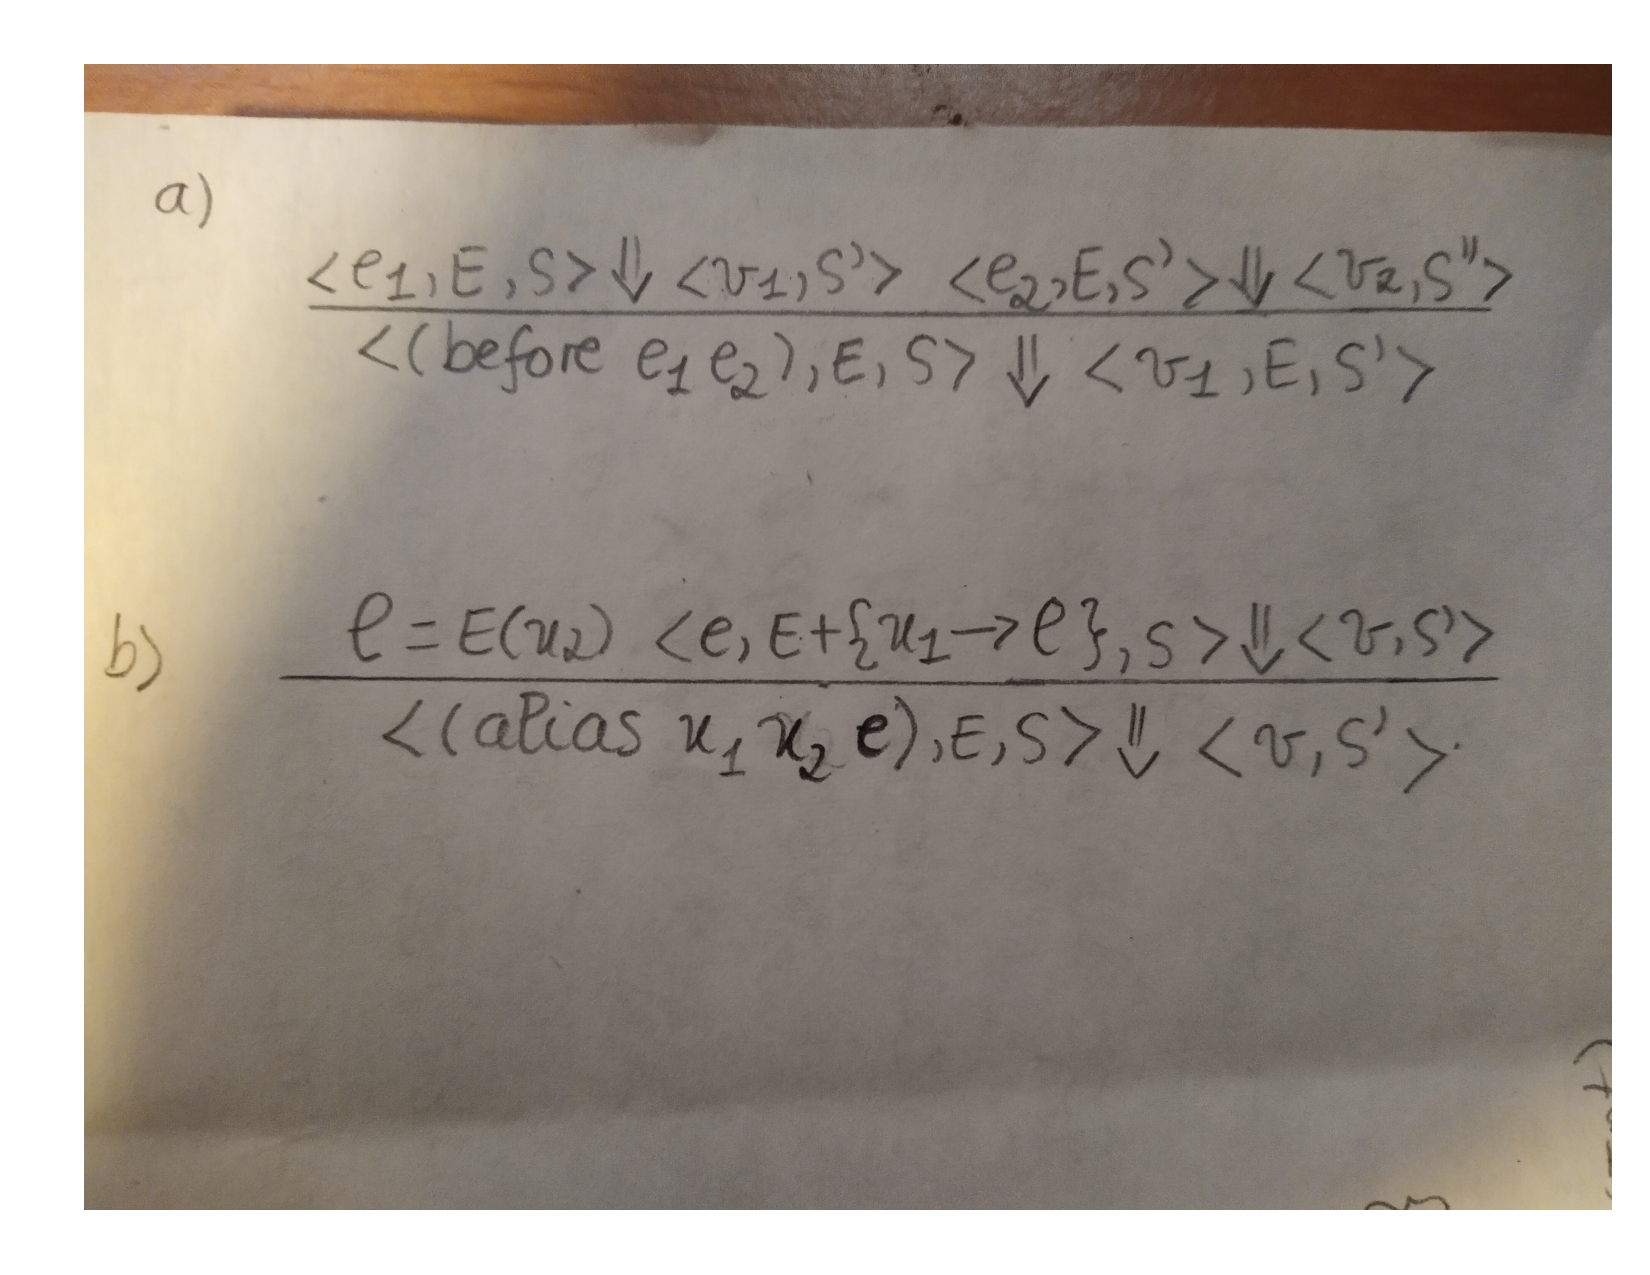
\includegraphics[width=\linewidth]{4.png}
					\captionof{figure}{Image after stegoDestroy}
				\end{minipage}
			
				
	
\end{document}